\documentclass[9pt]{article}

\usepackage[utf8]{inputenc}
\usepackage{geometry}
\geometry{
    a4paper,
    total={170mm,257mm},
    left=15mm,
    right=15mm,
    top=20mm,
    bottom=20mm,
}
\usepackage{multicol}
\usepackage[font=small,labelfont=bf]{caption}
\setlength{\columnsep}{0.25cm}
\usepackage[inline]{enumitem}
\usepackage{amssymb}
\usepackage{xcolor}
\usepackage{mathtools} 
\setlength{\parindent}{0em}
\setlength{\parsep}{0em}
\usepackage{tikz}
\setlength{\parskip}{0em}
\usetikzlibrary{decorations.pathmorphing,patterns}
\usepackage[american,cuteinductors]{circuitikz}
\usetikzlibrary{shapes,arrows,circuits,calc,babel}
% Definition of blocks:
\tikzset{%
  block/.style    = {draw, thick, rectangle, minimum height = 3em,
    minimum width = 3em},
  sum/.style      = {draw, circle, node distance = 2cm}, % Adder
  input/.style    = {coordinate}, % Input
  output/.style   = {coordinate} % Output
}
% Defining string as labels of certain blocks.
\newcommand{\suma}{\Large$+$}
\newcommand{\inte}{$\displaystyle \int$}
\newcommand{\derv}{\huge$\frac{d}{dt}$}

\def\mf{\ensuremath\mathbf}
\def\mb{\ensuremath\mathbb}
\def\mc{\ensuremath\mathcal}
\def\lp{\ensuremath\left(}
\def\rp{\ensuremath\right)}
\def\lv{\ensuremath\left\lvert}
\def\rv{\ensuremath\right\rvert}
\def\lV{\ensuremath\left\lVert}
\def\rV{\ensuremath\right\rVert}
\def\lc{\ensuremath\left\{}
\def\rc{\ensuremath\right\}}
\def\ls{\ensuremath\left[}
\def\rs{\ensuremath\right]}
\def\bmx{\ensuremath\begin{bmatrix*}[r]}
\def\emx{\ensuremath\end{bmatrix*}}
\def\bmxc{\ensuremath\begin{bmatrix*}[c]}
\def\emxc{\ensuremath\end{bmatrix*}}
% \def\t{\lp t\rp}
% \def\k{\ls k\rs}

\newcommand{\demoex}[2]{\onslide<#1->\begin{color}{black!60} #2 \end{color}}
\newcommand{\demoexc}[3]{\onslide<#1->\begin{color}{#2} #3 \end{color}}
\newcommand{\anim}[3]{\onslide<#1->{\begin{color}{#2!60} #3 \end{color}}}
\newcommand{\ct}[1]{\lp #1\rp}
\newcommand{\dt}[1]{\ls #1\rs}

\renewcommand{\familydefault}{\sfdefault}

\begin{document}
\begin{center}
\begin{Large}
\textbf{Linear Systems: Matrices Assignment}
\end{Large}
\end{center}
\vspace{0.2cm}

\begin{multicols}{2}
  \begin{enumerate}
    % \item Elements of the matrix $\mf{C} \in \mb{R}^{m \times n}$ obtained as the product of two matrices $\mf{A} \in \mb{R}^{m \times p}$ and $\mf{B} \in \mb{R}^{p \times n}$ is given by,
    % \[ c_{ij} = \sum_{k=1}^{p}a_{ik}b_{kj} \]
    % We had discussed four different ways to think of matrix multiplication. By algebraically manipulating the previous equation arrive at these four views (inner product view, column view, row view and outer product view)? 

    \item Given the matrices $\mf{A} = \begin{bmatrix*}[r]
    1 & 2 & 3 & 4\\
    -1 & 3 & -1 & -1\\
    2 & -2 & 0 & 2\\
    1 & 0 & -3 & 0\\
    \end{bmatrix*}$, $\mf{B} = \begin{bmatrix*}[r]
    -1 & 1\\
    0 & 1\\
    -1 & 1\\
    -0 & 1\\
    \end{bmatrix*}$ and $\mf{C} = \begin{bmatrix*}[r]
    1 & 1\\
    0 & 1\\
    \end{bmatrix*}$. Evaluate the following products.

    \begin{enumerate*}
        \item $\mf{AB}$
        \item $\mf{A}^2\mf{B}$
        \item $\mf{C}\mf{B}^T\mf{A}$
        \item $\mf{C}^3$
        \item $\mf{ABC}$
    \end{enumerate*}

    \item \textbf{Computational cost of different operations.} What is computational cost of the following matrix operations? Computational cost refers to the number of arithmetic operations  required to carry out a particular matrix operation. Computational cost is a measure of the efficiency of an algorithm. For example, the consider the operation of vector addition, $\mf{a} + \mf{b}$, where $\mf{a}, \mf{b} \in \mb{R}^n$. This requires $n$ addition/subtraction operations and zero multiplication/division operations.
    \begin{enumerate}
        \item Matrix multiplication: $\mf{AB}$, where $\mf{A}, \mf{B} \in \mb{R}^{n \times n}$
        \item Inner product: $\mf{u}^T\mf{v}$
        \item Gaussian Elimination for $\mf{A}\mf{x} = \mf{b}$ where $\mf{A} \in \mb{R}^{n \times n}$, $\mf{x}, \mf{b} \in \mb{R}^{n}$.
        \item Back substitution
        \item Gauss-Jordan method to obtain the row echelon form: $\mf{A} \longrightarrow \mf{E}$.
        \item Matrix inversion using the Gauss-Jordan method: $\bmx \mf{A} \vert \mf{I} \emx \longrightarrow \bmx \mf{I}\vert\mf{A}^{-1}\emx$
    \end{enumerate} 
    Report the counts for the addition/subtraction and multiplication/division operations separately. 

    \item Prove $\ct{\mf{A}\mf{B}}^T = \mf{B}^T\mf{A}^T$.

    \item Consider the following matrix,
    \[ \mf{A} = \bmx \frac{\sqrt{3}}{2} & -\frac{1}{2}\\\frac{1}{2} & \frac{\sqrt{3}}{2} \emx \bmx 0.1 & 0\\0 & 0.9 \emx \bmx \frac{\sqrt{3}}{2} & \frac{1}{2}\\-\frac{1}{2} & \frac{\sqrt{3}}{2} \emx \]
    Find out the expression for $\mf{A}_n = \mf{A}^n$. What is $\mf{A}_\infty = \lim_{n\to\infty} \mf{A}^n$?

    \item Derive force and displacement relationship for a series of $n+1$ springs (with spring constants $k_i$) connected in a line. There are $n$ nodes, with $f_i$ and $x_i$ representing the force applied and resulting displacement at the $i^{th}$ node. 
    \begin{center}
        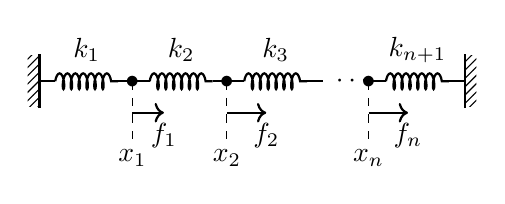
\begin{tikzpicture}
            \fill [pattern = north east lines] (-0.15,-0.325) rectangle (0,0.325);
            \draw[thick] (0,-0.34) -- (0,0.34);

            \draw[thick] (0,0) -- (0.2,0);
            \draw[decoration={aspect=0.3, segment length=1mm, amplitude=1mm, coil,},decorate, thick] (0.2,0) -- (1.0,0);
            \draw[thick] (1.0,0) -- (1.2,0);
            \node[black] at (1.18,-0.02) {$\bullet$};
            \node[black] at (0.6,0.4) {$k_1$};
            \draw[dashed, thin] (1.18,0) -- (1.18,-0.75) node[below]{$x_1$};
            \draw[->,thick] (1.18,-0.4) -- (1.58,-0.4) node[below]{$f_1$};

            
            \draw[thick] (1.2,0) -- (1.4,0);
            \draw[decoration={aspect=0.3, segment length=1mm, amplitude=1mm, coil,},decorate, thick] (1.4,0) -- (2.2,0);
            \draw[thick] (2.2,0) -- (2.4,0);
            \node[black] at (2.38,-0.02) {$\bullet$};
            \node[black] at (1.8,0.4) {$k_2$};
            \draw[dashed, thin] (2.38,0) -- (2.38,-0.75) node[below]{$x_2$};
            \draw[->,thick] (2.38,-0.4) -- (2.88,-0.4) node[below]{$f_2$};
            
            \draw[thick] (2.4,0) -- (2.6,0);
            \draw[decoration={aspect=0.3, segment length=1mm, amplitude=1mm, coil,},decorate, thick] (2.6,0) -- (3.4,0);
            \draw[thick] (3.4,0) -- (3.6,0);
            \node[black] at (3.0,0.4) {$k_3$};

            \node[black] at (4.0, 0) {$\cdots$};

            \draw[thick] (4.2,0) -- (4.4,0);
            \draw[decoration={aspect=0.3, segment length=1mm, amplitude=1mm, coil,},decorate, thick] (4.4,0) -- (5.2,0);
            \draw[thick] (5.2,0) -- (5.4,0);
            \node[black] at (4.18,-0.02) {$\bullet$};
            \node[black] at (4.8,0.4) {$k_{n+1}$};
            \draw[dashed, thin] (4.18,0) -- (4.18,-0.75) node[below]{$x_n$};
            \draw[->,thick] (4.18,-0.4) -- (4.68,-0.4) node[below]{$f_n$};

            \fill [pattern = north east lines] (5.4,-0.325) rectangle (5.55,0.325);
            \draw[thick] (5.4,-0.34) -- (5.4,0.34);
        \end{tikzpicture}
    \end{center}
    \begin{enumerate}
        \item Represent the relationship in the following form,
        \[ \mf{f} = \mf{Kx}; \,\,\, \mf{f} = \begin{bmatrix}f_1\\ f_2\\ \vdots\\ f_n\end{bmatrix}; \,\,\, \mf{x} = \begin{bmatrix}x_1 \\ x_2 \\ \vdots \\ x_n\end{bmatrix}\]
        \item What kind of a pattern does $\mf{K}$ have?
        \item Consider a specific case where $n = 4$ and $k = 1.5 N.m^{-1}$. What should be forces applied at the four nodes in order to displace the spring $\mf{x} = \begin{bmatrix*} 0.5 \\ -0.5 \\ 0 \\ 0 \end{bmatrix*}m$. 
    \end{enumerate}

    \item Prove that a matrix $\mf{M} \in \mathbb{R}^{n \times n}$ can always be written as a sum a symmetric matrix $\mf{S}$ and a skew-symmetric matrix $\mf{A}$.
    \[ \mf{M} = \mf{S} + \mf{A}, \,\,\, \mf{S}^T = \mf{S} \, \text{ and } \, \mf{A}^T = -\mf{A} \]

    Does this property also hold for a complex matrix $\mf{M} \in \mb{C}^{n \times n}$?
    \item The trace of a matrix $\mf{A} \in \mb{R}^{n \times n}$ is defined as, $trace\left(\mf{A}\right) = \sum_{i=1}^{n}a_{ii}$. Prove the following,
    \begin{enumerate}
        \item $trace\left(\mf{A}\right)$ is a linear function of $\mf{A}$.
        \item $trace\left(\mf{AB}\right) = trace\left(\mf{BA}\right)$
        \item $trace\left(\mf{A}^T\mf{A}\right) = 0 \implies \mf{A} = 0$
    \end{enumerate}

    \item Prove that the rank of an outer product $\mf{x}\mf{y}^T$ is 1, where $\mf{x},\mf{y} \in \mb{R}^n$ and $\mf{x}, \mf{y} \neq \mf{0}$.

    \item Is there a relationship between the space of solutions to the following two equations? 
    \[ \mf{y}^T\mf{A} = \mf{c}^T \,\,\,\, \text{ and } \,\,\,\,\, \mf{A}\mf{x} = \mf{b} \]
    If so, how are they related?
    
    \item Consider an upper triangular and lower triangular matrices $\mf{U}$ and $\mf{L}$, respectively. 
    \begin{enumerate}
        \item Is the product of two upper triangular matrices $\mf{U}_1\mf{U}_2$ upper triangular?
        \item Is the product of two lower triangular matrices $\mf{L}_1\mf{L}_2$ upper triangular?
        \item What is the $trace\lp \mf{L}\mf{U} \rp$?
    \end{enumerate}

    \item Consider the following electrical circuit with rectangular grid of resistors $R$. The input to this grid is a set of current injected at the top node as shown in the figure, such that $\sum_{k=1}^5i_k = 0$.
    \vspace{-0.25cm}
    \begin{center}
    \begin{circuitikz}[scale=0.9]
        \draw (2,0) to[R,*-*] (0,0)
        to[R,*-*] (0,2) to[R,*-*] (0,4) to[R,*-*] (2,4)
        to[R,*-*] (2,2) to[R,*-*] (2,0) to[R,*-*] (4,0)
        to[R,*-*] (4,2) to[R,*-*] (4,4) to[R,*-*] (6,4)
        to[R,*-*] (6,2) to[R,*-*] (6,0) to[R,*-*] (8,0)
        to[R,*-*] (8,2) to[R,*-*] (8,4) to[R,*-*] (6,4);

        \draw (0,2) to[R,*-*] (2,2);
        \draw (2,4) to[R,*-*] (4,4);
        \draw (2,2) to[R,*-*] (4,2);
        \draw (4,2) to[R,*-*] (6,2);
        \draw (4,0) to[R,*-*] (6,0);
        \draw (6,2) to[R,*-*] (8,2);

        \draw (0,5) node[above]{$i_1$} to[short, o-] (0,4);
        \draw (2,5) node[above]{$i_2$} to[short, o-] (2,4);
        \draw (4,5) node[above]{$i_3$} to[short, o-] (4,4);
        \draw (6,5) node[above]{$i_4$} to[short, o-] (6,4);
        \draw (8,5) node[above]{$i_5$} to[short, o-] (8,4);
     \end{circuitikz}
     \end{center}

     Express the relationship between the voltages at the different nodes (represented by $\bullet$ in the figure) and the net current flowing in/out of the node in the following form, $\mf{G}\mf{v} = \mf{i}$. Where, $\mf{G}$ is the conductance matrix, $\mf{v}$ is the vector of node voltages, and $\mf{i}$ is the vector representing the net current flow in/out of the different node.

    \item Consider the square full rank matrix $\mf{A}$, and let the $\mf{x}_i$ be then solution to the equation $\mf{A}\mf{x}_i = \mf{e}_i$. Show that the matrix $\mf{X} = \bmx \mf{x}_1 & \mf{x}_2 & \ldots & \mf{x}_n \emx$ is the inverse of $\mf{A}$.

    % \item How many different reduced row echelon forms can a matrix $\mf{A} \in \mb{R}^{4 \times 5}$ have? Hint: \emph{Think in terms of basic and non-basic columns.}

    \item Consider the system of equation, $\mf{Ax} = \mf{b}$, such that a matrix $\mf{A} \in \mb{R}^{m \times n}$, $\mf{x}, \mf{b} \in \mb{R}^n$. Are the following statements true? Explain your answer.
    \begin{enumerate}
        \item $rank \lp \mf{A} \rp \leq \min \lp m, n \rp$
        \item The system is consistent if $\,rank\lp \mf{A} \rp = m$.
        \item The system has a unique solution if $\,rank \lp \mf{A} \rp = n$.
    \end{enumerate}

    \item Consider a linear function $f: V \to W$, where $V \subset \mb{R}^n$ and $W \subset \mb{R}^m$. If $V$ is a subspace of $\mb{R}^n$ then prove that $W$ is a subspace of $\mb{R}^m$.   

    \item For a $n \times n$ square matrix $\mf{A}$, prove that if $\mf{A}\mf{X} = \mf{I}$, then $\mf{X}\mf{A} = \mf{I}$ and $\mf{X} = \mf{A}^{-1}$.

    \item If two systems of linear equations are consistent, with augmented matices $\left[ \mf{A} | \mf{b}\right]$ and $\left[ \mf{A} | \mf{c}\right]$. Is $\left[ \mf{A} | \mf{b} + \mf{c}\right]$ consistent?

    \item Prove the following for the non-singular square matrices $\mf{A}$ and $\mf{B}$:
    \begin{enumerate}
        \item $\mf{A}\mf{B}$ is non-singular.
        \item $\ct{\mf{A}^{-1}}^{-1} = \mf{A}$.
        \item $\ct{\mf{A}\mf{B}}^{-1} = \mf{B}^{-1}\mf{A}^{-1}$
        \item $\ct{\mf{A}^T}^{-1} = \ct{\mf{A}^{-1}}^T$
    \end{enumerate}

    % \item If a matrix $\mf{A}$ has LU decomposition, such that $\mf{A} = \mf{LU}$. Demonstrate that it also has a LDU decomposition $\mf{A} = \mf{LD}\hat{\mf{U}}$, where $\mf{D}$ is a diagonal matrix, and $\hat{\mf{U}}$ is upper triangular. What happens to the LU and LDU decompositions when a matrix $\mf{A} = \mf{A}^T$?

    % \item Write down a basis for the four fundamental subspaces of the following matrix,
    % \[ \mf{A} = \begin{bmatrix*}[r]
    % 1 & 2 & -3 & 4 & -1 & 0 \\
    % 4 & 8 & 12 & -8 & 2 & 1 \\
    % 2 & 3 & 2 & 1 & -2 & 0 \\
    % -3 & -1 & 1 & -4 & 0 & -1 \\
    % 1 & -2 & -1 & 0 & 0 & 0 \\
    % \end{bmatrix*} \]
    
    % \item Consider a matrix $\mf{A} = \begin{bmatrix*}[r] 1 & 4 & 5\\ 4 & 118 & 26\\3 & 16 & 30\end{bmatrix*}$.
    % \begin{enumerate}
    %     \item Apply Gaussian elimination to simply this matrix into an upper-triangular matrix $\mf{U}$.
    %     \item What is the corresponding upper-triangular matrix $\tilde{\mf{U}}$ obtained by applying Gaussian elimination to $\mf{A}^T$? 
    %     \item Could you have arrived at $\tilde{\mf{U}}$ without having to repeat the Gaussian elimination process on $\mf{A}^T$?
    %     \item Write down the LDU decompositions of $\mf{A}$ and $\mf{A}^T$.
    % \end{enumerate} 

    \item Derive the inverse of the matrix $\mf{A} = \begin{bmatrix}a & b\\c & d\end{bmatrix}$.
    
    \item Consider the following upper-triangular matrix, 
    $$U = \begin{bmatrix}
    u_{11} & u_{12} & u_{13} & \cdots & u_{1n}\\
    0 & u_{22} & u_{23} & \cdots & u_{2n}\\
    0 & 0 & u_{33} & \cdots & u_{3n}\\
    \vdots & \vdots & \vdots & \ddots & \vdots\\
    0 & 0 & 0 & \cdots & u_{nn}\\\end{bmatrix}$$
    where, $u_{ii} \neq 0, \,\,\, 1 \leq i \leq n$. Do the columns of this matrix form a linearly independent set? Explain your answer.

    \item Verify that $\mf{A}$ and $\mf{B}$ are inverses of each other,
    \begin{enumerate}
        \item $\mf{A} = \mf{I} - \mf{u}\mf{v}^T$ and $\mf{B} = \mf{I} + \mf{u}\mf{v}^T / \lp 1 - \mf{v}^T\mf{u} \rp$
        \item $\mf{A} = \mf{C} - \mf{u}\mf{v}^T$ and $\mf{B} = \mf{C}^{-1} + \mf{C}^{-1}\mf{u}\mf{v}^T\mf{C}^{-1} / \lp 1 - \mf{v}^T\mf{C}^{-1}\mf{u} \rp$
        \item $\mf{A} = \mf{I} - \mf{U}\mf{V}$ and $\mf{B} = \mf{I}_{n} + \mf{U}\lp \mf{I}_m - \mf{V}\mf{U}\rp^{-1}\mf{V}$
        \item $\mf{A} = \mf{C} - \mf{U}\mf{D}^{-1}\mf{V}$ and $\mf{B} = \mf{A}^{-1} + \mf{A}^{-1}\mf{U}\lp \mf{D} - \mf{V}\mf{A}^{-1}\mf{U}\rp^{-1}\mf{V}\mf{A}^{-1}$
    \end{enumerate}
    where, $\mf{A}, \mf{B} \in \mb{R}^{n \times n}$, $\mf{u}, \mf{v} \in \mb{R}^n$, $\mf{U} \in \mb{R}^{n \times m}$, $\mf{V} \in \mb{R}^{m \times n}$ and $\mf{D} \in \mb{R}^{m \times m}$.

    \item Consider the matrices $\mf{A} \in \mb{R}^{m \times m}$, $\mf{B} \in \mb{R}^{n \times n}$ and $\mf{C} \in \mb{R}^{m \times n}$. Verify the following,
    \begin{enumerate}
        \item $\bmx \mf{A} & \mf{0} \\ \mf{0} & \mf{B}\emx^{-1} = \bmx \mf{A}^{-1} & \mf{0} \\ \mf{0} & \mf{B}^{-1}\emx$
    \end{enumerate}
    
    % \item Gaussian elimination does not change the solution of a system $\mf{A}\mf{x} = \mf{b}$. Explain why the three row operations do not affect the solution of the system. Instead of row operations, what if we performed column operations. Will the solution of the system $\mf{Ax} = \mf{b}$ still remain unchanged? If the solution is affected, how is it affected by the following operations?
    % \begin{enumerate}
    %     \item Columns $\mf{a}_i$ and $\mf{a}_j$ of $\mf{A}$ are interchanged.
    %     \item Column $\mf{a}_i$ is replaced by $\alpha\mf{a}_i$.
    %     \item Columns $\mf{a}_i$ is replace by $\mf{a}_i + \beta\mf{a}_j$.
    % \end{enumerate}

    \item \textbf{Two point boundary problem.} $\mf{A}\mf{x} = \mf{b}$ is often encountered in many practical applications. One such application is the numerical solution of differential equations of the following form,
    \[ \sum_{i=0}^M a_{i}\ct{x}y^{\ct{i}}\ct{x} = f\ct{x} \]
    where, $x \in \dt{a, b}$ and $y\ct{a} = \alpha, y\ct{b} = \beta$. 

    Numerical methods are often employed for obtaining an approximate estimate of $y\ct{x}$ at discrete points in the interval $\dt{a,b}$. The interval is divided into subintervals of width $\Delta x$. The derivate of $y\ct{x}$ at the different nodes (points between two subintervals) can be approximated as the following,
    \begin{align}
    y'\ct{x_i} &= \frac{y\ct{x_i + \Delta x} - y\ct{x_i - \Delta x}}{\Delta x}\nonumber\\
    y''\ct{x_i} &= \frac{y\ct{x_i + \Delta x} + 2y\ct{x_i} - y\ct{x_i - \Delta x}}{\Delta x^2} \nonumber
    \end{align}
    where, $x_i = a + i\Delta x, \,\, 0 \leq i \leq N+1$, and $b - a = \ct{N+1} \Delta x$. Addition and subtracting the above two equations and neglecting terms involving higher orders of $\Delta x$, we get the following approximations for the derivatives of $y\ct{x}$ at $x_i$.

    Replacing the derivatives of $y\ct{x}$ by the above approximations and evaluating the equation at the different nodes $x_i$s, we arrive a set of $N$ linear equations with $N$ unknowns $y\ct{x_1}, y\ct{x_2}, \ldots y\ct{x_N}$. 

    Using this approach, compute an approximate solution for $y\ct{x}$ for the following differential equations over the interval $x \in \dt{0, 1}$. 
    \begin{enumerate}
         \item $y''\ct{x} = -x$
         \item $y''\ct{x} + y'\ct{x} = x$
    \end{enumerate}
    Solve these equations for different values of $\Delta x$, and compare the resulting approximate solution for $y\ct{x}$ with the exact solution.   Present your results as a plot the solution $y\ct{x_i}$ versus $x_i$.

    Comment on the dependence of the solution $\ct{x}$ on $\Delta x$. What is the best value for $\Delta x$ to use in solving these equations?

    \item \label{matrices:uncertain} \textbf{Ill-conditioned systems.} A system $\mf{A}\mf{x} = \mf{b}$ is said to be ill-conditioned when small changes in the components of $\mf{A}$ or $\mf{b}$ can produce large changes in the solution $\mf{x}$. Consider the following system,
    \begin{align}
    x - y &= 100 \nonumber \\
    10 + \ct{9 + \Delta}y &= 0 \nonumber
    \end{align}
    Find the solutions of the system for different values of $\Delta = -2, -1, 0, 1, 2$. How do the solutions change with $\Delta$. Now consider the following system,
    \begin{align}
    x - y &= 100 \nonumber \\
    10 - \ct{9 + \Delta}y &= 0 \nonumber
    \end{align}
    The second system is an example of an ill-conditioned system. What can you say about the geometries of these two systems?

    \item \textbf{Connectivity matrices.} Another common application of matrices is in graph theory. A graph is a set of vertices or nodes connected by edges, as show in the following figure. $A$-$F$ are the nodes of the graph, and the lines with the arrows are the edges that convey information about the connections or relationships between the nodes.
    \begin{center}
        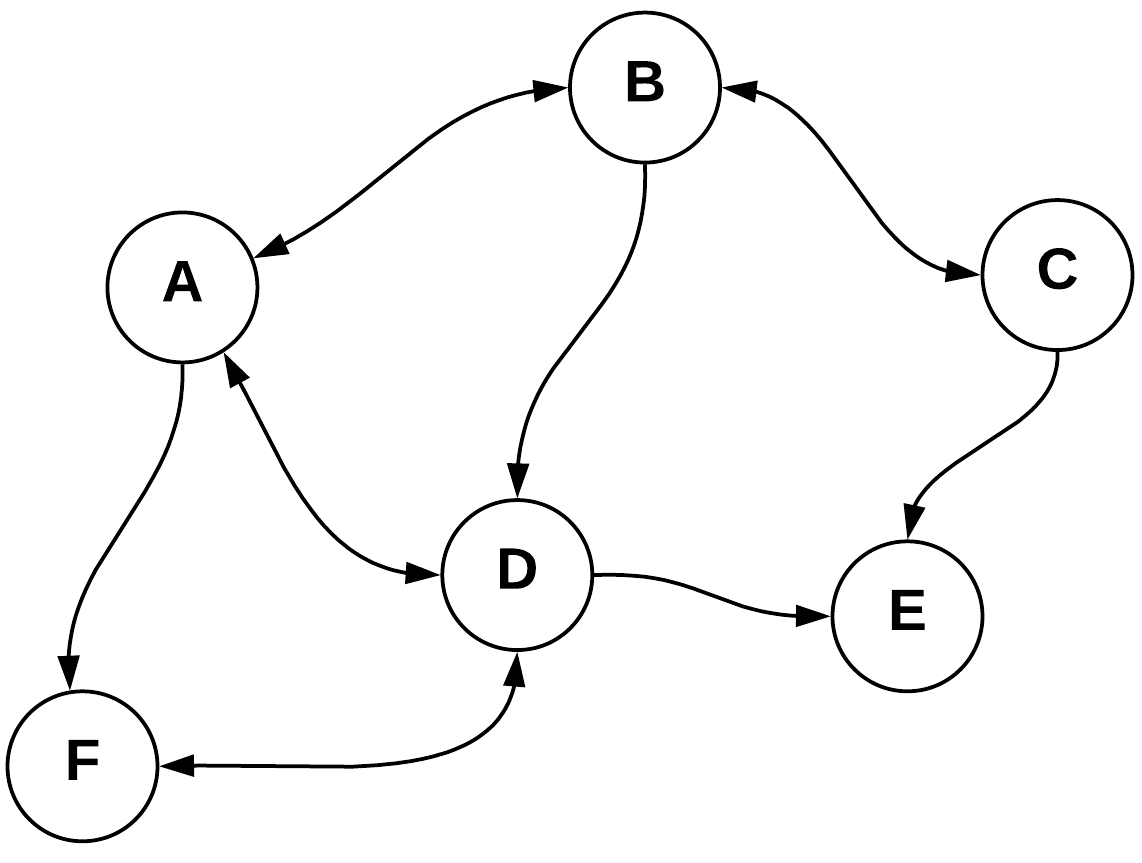
\includegraphics[width=0.5\columnwidth]{../figs/graph.png}
    \end{center}
    The above graph can be thought as a representation of different places in a city (represented by the nodes), and the lines with the arrows represent the roads connecting these different places. A line with two arrows allow two-way traffic, while line with single arrow only allow one way traffic. The connectivity between the different places can be summarized though the connectivity matrix $\mf{C} \in \mb{R}^{n \times n}$, where $n$ is the number of nodes in the graph. The elements of this connectivity matrix  represents whether or not there is a direct path between two places.
    \[ 
    c_{ij} = \begin{cases}
        1 & \text{there is a direct road between places } i \, \& \,j. \\
        0 & \text{otherwise.}
    \end{cases}
    \]
    The diagonal element of $\mf{C}$ are zero, $c_{ii} = 0$.

    Write down the connectivity matrix $\mf{C}$ for the graph shown above. How can we use the matrix $\mf{C}$ to answer the following questions? Explain exact matrix operation you would perform to answer these questions (Hint: Consider higher power of $\mf{C}$).
    \begin{enumerate}
        \item Is there a path between two places $i$ and $j$ that goes via one other place? For example, we can go from $A$ to $D$ via $B$.
        \item How many paths are there between places $i$ and $j$ that goes via three other places?
    \end{enumerate}
\end{enumerate}

\end{multicols}
\end{document}